\chapter{State of the Art}
\chaptermark{State of the Art}
\label{chapter:soa}
\minitoc

%%%%%%%%%%%%%%%%%%%%%%%%%%%%%%%%%%%%%%%%%%%%%%%%%%%%%%%%%%%%%%%%%%%%%%%%%%%%%%%%%%%%%%%%%%%%%%%
\section{Introduction}
This chapter provides an overview of related work to contextualize the primary objectives of this thesis. Firstly, in Section~\ref{section:ift}, Information Flow Tracking (IFT) is introduced, detailing the different types and their respective purposes. We will discuss the various levels of monitoring, from program behaviour to the detection of hardware trojans.
Then in Section~\ref{section:physicalAttacks}, Physical Attacks are examined, focusing on two main types: Side-Channel Attacks (SCA) and Fault Injection Attacks (FIA).
Finally in Section~\ref{section:countermeasuresAgainstFIA}, as this work will concentrate on FIA, we will exclusively present countermeasures against Fault Injection Attacks.

%%%%%%%%%%%%%%%%%%%%%%%%%%%%%%%%%%%%%%%%%%%%%%%%%%%%%%%%%%%%%%%%%%%%%%%%%%%%%%%%%%%%%%%%%%%%%%%
\section{Information Flow Tracking}
\label{section:ift}
The concept of \textit{Information Flow Tracking} has been introduced by the work of Bell and LaPadula~\cite{BLP-76-military} and by Denning~\cite{D-76-commacm} in 1976.
This section introduces Information Flow Tracking mechanisms, explains how they work, and presents the various types of IFT with their different functional levels.
    
%%%%%%%%%%%%%%%%%%%%%%%%%%%%%%%%
\subsection{Different types of IFT}
There are two distinct types of IFT approaches: static and dynamic, each with its own specific objectives.

\subsubsection{Static IFT}
Static Information Flow Tracking (SIFT) is a security technique used to analyse and control the flow of information within a program or system without executing it, by examining the source code or compiled binary~\cite{HAK-21-acmcsur}. This method is particularly useful for identifying theoretical vulnerabilities, ensuring compliance with design principles, and preventing unauthorised information leaks before deployment. SIFT is comprehensive, covering all possible execution paths and detecting both explicit information flows (direct data assignments) and implicit flows (leaks through control flow structures). By performing checks at compile-time, SIFT helps developers address potential security issues early, enforcing principles like non-interference and data confidentiality through security policies. However, static analysis may generate false positives by flagging theoretical flows that might not occur in practice and may struggle with certain dynamic language features or runtime-dependent behaviours. SIFT is employed in various contexts, such as verifying secure information flow in operating systems, programming languages with built-in information flow controls, and hardware design for secure systems.

\subsubsection{Dynamic IFT}
Dynamic Information Flow Tracking (DIFT) is a powerful security technique that monitors and analyses, in real-time, the flow of information within a program during its execution~\cite{CGDJ-21-micromac}. DIFT operates by tagging or labelling input data from potentially untrusted sources and tracking how this data propagates through the system~\cite{SLD-04-sigplan}. As the program executes, DIFT maintains metadata about the tagged information, updating it as operations are performed on the data. This allows the system to detect when tainted data is used in security-critical operations, such as modifying control flow or accessing sensitive resources. DIFT can be implemented at various levels, including hardware, software, or a combination of both. Hardware-based implementations often offer better performance but require specialized processor modifications, while software-based approaches provide more flexibility but may incur higher overhead~\cite{CGDJ-21-micromac}. DIFT has proven effective in detecting and preventing a wide range of security vulnerabilities, including buffer overflows, format string attacks, and code injection attacks~\cite{SLD-04-sigplan}. However, DIFT also faces challenges, such as handling implicit information flows, managing performance overhead, and addressing over-tainting issues.
This approach might not cover all potential data paths, as it is dependent on the specific conditions and inputs provided during the monitoring period.
Despite these challenges, DIFT remains a valuable tool for software security, particularly for runtime attack detection in modern systems.

%%%%%%%%%%%%%%%%%%%%%%%%%%%%%%%%    
\subsection{Different levels of DIFT}
IFT can be implemented at various levels of abstraction in computing systems~\cite{HAK-21-acmcsur, BSMCVEJCO-21-acmcsur,CGDJ-21-micromac}. Each level presents unique trade-offs between precision, performance overhead, and ease of implementation, allowing designers to choose the most appropriate approach for their security requirements.

Software-based DIFT mechanisms benefit from close integration with the software context via binary code instrumentation and source code modifications, offering better flexibility, customisation, and scalability without altering hardware components. However, these software solutions often incur high performance overheads due to the extra instructions required. They operate at either the system level, monitoring OS-wide information flows, or the program level, focusing on specific applications.
On the other hand, hardware-assisted DIFT designs can efficiently enforce security rules by implementing DIFT-related operations as hardware logic, reducing performance overhead but at the expense of flexibility and scalability, making them challenging to deploy in modern commercial systems. They can be implemented within processor cores or as off-core designs. But they can also be at the lowest level such as Gate-Level IFT who tracks information flow through logic gates.
A hybrid hardware and software co-design offers a promising alternative, enabling fine-grained security checks by associating software context with hardware data, though it faces challenges such as balancing flexibility with hardware overhead and designing appropriate tags that support rule updates post-deployment.


Figure~\ref{fig:levels_system} represents the different levels of a simplified embedded system: application layer, system service layer, OS layer, and hardware layer. This figure is inspired by Figure 1.9 of~\cite{ebrary}. Software-based IFTs work in the first three levels.

Positioned at the highest level of the software hierarchy, \textit{the application layer} is responsible for implementing system functionalities and business logic. Functionally, all modules within this layer work together to execute the required system operations. Applications generally run in a less-privileged mode on the processor and utilise the OS-provided API scheduling to communicate with the operating system.
\textit{The system service layer} serves as the intermediary service interface offered by the OS to the application layer. This interface allows applications to access a variety of OS-provided services, essentially bridging the gap between the OS and applications. Typically, this layer encompasses components like the file system, Graphical User Interface (GUI), task manager.
An Operating System (OS) is a software framework designed to manage hardware resources uniformly. It abstracts numerous hardware functions and offers them to applications as services. Common services provided by an OS include scheduling, file synchronisation, and networking. Operating systems are prevalent in both desktop and embedded systems. In the context of embedded systems, OSs possess distinct characteristics such as stability, customisability, modularity, and real-time processing capabilities.
\textit{The hardware layer} refers to the physical components and circuitry, including the microprocessor or microcontroller, memory, sensors, and input/output interfaces. This layer encompasses all the tangible electronic elements that interact directly with each other to perform the device's functions. It provides the essential infrastructure that supports and drives the embedded system’s operations and connectivity.

\begin{figure}[ht]
    \centering
    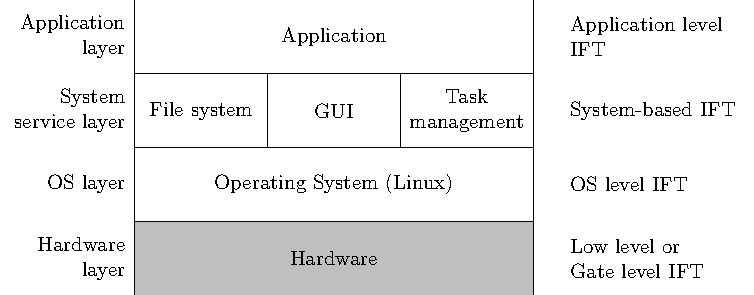
\includegraphics{c2_soa/img/system_layer.pdf}
    \caption{Simplified representation of the different layers in an embedded system}
    \label{fig:levels_system}
\end{figure}

Tracking information can be performed at various levels, from the application level to the hardware level. Each level offers distinct advantages and disadvantages.
For instance, application-level tracking might provide detailed insights and user-friendly interfaces, while hardware-level tracking offers more granular data and real-time monitoring but can be more complex and costly.
The following subsections will explore these different levels, highlighting their respective benefits and limitations.


\subsubsection{Software-based DIFT}
\paragraph{Application level DIFT} tracks information flows between application variables. The programmer has to integrate data tagging inside his program and use a modified compiler or analyse his program to check if no security violation happened.
One application for DIFT at application level is language-based. Several security extensions have been proposed for existing programming languages.
JFlow~\cite{M-99-popl} is one of the first works that has described an extension of the Java language by adding statically-checked information flow annotations.

Multiples works introduce DIFT extensions for different languages, for example such as JavaScript~\cite{CN-15-ccs, AF-09-plas}.
Austin et al.~\cite{AF-09-plas} propose a method for tracking information flow in dynamically-typed languages, focusing on addressing issues with implicit paths through a dynamic check. This approach avoids the necessity for approximate static analyses while still ensuring non-interference. The method employs sparse information labelling, keeping flow labels implicit where possible and introducing explicit labels only for values crossing security domains.

Kemerlis et al.~\cite{KPJK-12-sigplan} provide a framework, \textit{libdft}, which is fast and reusable and applicable to software and hardware. \textit{libdft} provides an API for building DFT-enabled tools that work on unmodified binaries.

\paragraph{OS level and System-based DIFT} track and tag files (read or written) used by the application.
The main advantage of this approach is that it reduces the number of information flows which lead to an improvement of the runtime overhead. In the other side, the main disadvantage of this approach is that it results in more false positives than the application-level approach.

TaintDroid~\cite{EGHTCCJMS-14-tocs} introduces an extension to the Android mobile phone platform designed to monitor the flow of privacy-sensitive data through third-party applications. Operating under the assumption that downloaded third-party applications are untrusted, TaintDroid tracks in real-time how these applications access and handle users’ personal information. The primary objectives are to detect when sensitive data is transmitted out of the system by untrusted applications and to enable phone users or external security services to analyse these applications. They store the data adjacent to data for spatial locality. This may cause large performance and storage overheads, as the tag fetching requires extra clock cycles for memory access.
HiStar~\cite{ZBKM-11-commacm} is a new OS that has been designed to provide precise data specific security policies. The authors made the choice to assign tags to different objects in the operating system instead of data.


\subsubsection{Software and Hardware Co-Design-Based DIFT}
\wip{TODO}

\subsubsection{Hardware-based DIFT}
Dalton et al.~\cite{DKK-07-sigarch} report that software DIFT solutions add significative runtime overhead, up to a slow down of 37 times ! Therefore, in order to improve the execution time to be more on-the-fly, the idea is to implement directly the DIFT into the hardware, but at the expense of flexibility.
This subsection discusses the hardware-based DIFT designs including gate-level DIFT designs and micro-architecture-level DIFT designs. Surveys~\cite{HAK-21-acmcsur,BSMCVEJCO-21-acmcsur} present an overview on all hardware DIFT techniques. They developed a taxonomy for them and use it to classify and differentiate hardware DIFT tools and techniques.

\paragraph{Gate-Level DIFT} include gate-level netlist and also RTL designs. The goal is to protect against hardware trojans and unauthorized behaviors. To achieve that, during the creation of the circuit, additional logic is added for each gate used in the design.

GLIFT~\cite{TWMMCS-09-asplos} is a well-established IFT technique. The goal is to protect against hardware trojans and unauthorized behaviors. All information flows, both explicit and implicit, are unified at the gate level. GLIFT employs a detailed initialisation and propagation policy to precisely track each bit of information flow, by adding additional logic for each gate used in the design. By analysing how inputs influence outputs, GLIFT accurately measures true information flows and substantially reduces the false positives typically associated with conservative IFT techniques.
Hu et al.~\cite{HOITSMK-11-tcad} established the theoretical foundation for GLIFT. They introduced several algorithms for generating GLIFT logic in large digital circuits. Additionally, the authors identified the primary source of precision discrepancies in GLIFT logic produced by various methods as static logic hazards or variable correlation due to reconvergent fanouts. Many other works have been done on GLIFT to attempt a decrease of the logic complexity.

\paragraph{Off-Core DIFT} operations are performed on a dedicated processor working in parallel of the main core.
This approach needs a support from the OS for the synchronisation between data computations and tags computations in order to stall one core if it needs to wait the other.

Figure~\ref{fig:offcore_dift} represent how an off-core DIFT would be implemented. This Figure comes from article~\cite{KDK-09-dsn}. Authors of this paper, Kannan et al., described one of the first work using a coprocessor to improve tag computation runtime overhead. Traditional hardware DIFT systems require significant modifications to the processor pipeline, which increases complexity and design time.
This coprocessor handles all DIFT functionalities, synchronizing with the main processor only during system calls. This design eliminates the need for changes to the processor's pipeline, logic, or caches, making it more attractive. The coprocessor is small, with an area footprint of about 8\% of a simple RISC core, and introduces less than 1\% runtime overhead for SPECint2000 applications benchmark.
% The paper demonstrates that the coprocessor provides the same security guarantees as integrated DIFT architectures, supporting multiple security policies and protecting various memory regions and binary types. The authors present a prototype using a SPARC core, showing that the coprocessor can protect real-world Linux applications from both low-level and high-level security attacks with minimal performance impact. 
% This approach offers a balanced solution in terms of performance, cost, complexity, and practicality compared to existing DIFT implementations.

\begin{figure}[ht]
    \centering
    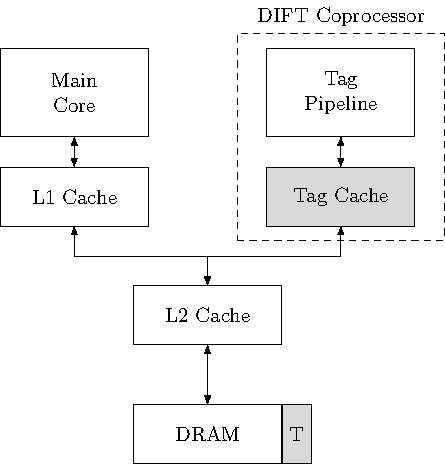
\includegraphics{c2_soa/img/offcore.pdf}
    \caption{Representation of an Hardware Off-Core DIFT (inspired by Figure 1 of~\cite{KDK-09-dsn})}
    \label{fig:offcore_dift}
\end{figure}

Wahab et al.~\cite{WCAHBLG-18-reconfig,WCAHLG-17-fpl}


\paragraph{Off-Loading DIFT}

Figure~\ref{fig:offloading_dift}

\begin{figure}[ht]
    \centering
    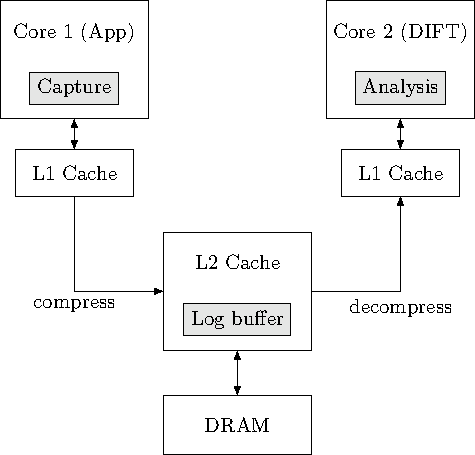
\includegraphics{c2_soa/img/offloading.pdf}
    \caption{Representation of an Hardware Off-Loading DIFT (inspired by Figure 1 of~\cite{KDK-09-dsn})}
    \label{fig:offloading_dift}
\end{figure}




\paragraph{In-Core DIFT}

Figure~\ref{fig:incore_dift}

\begin{figure}[ht]
    \centering
    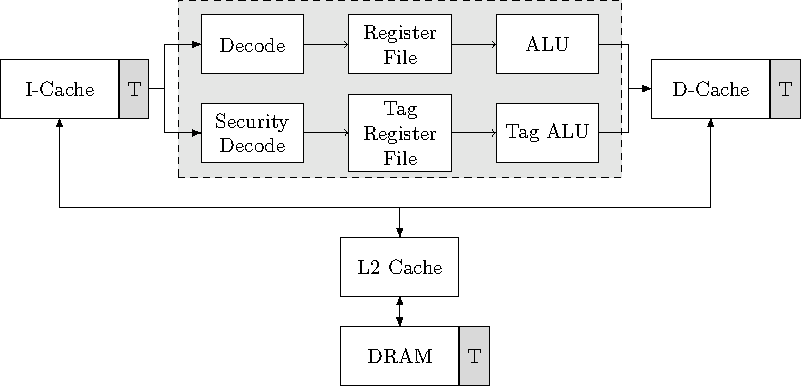
\includegraphics{c2_soa/img/incore.pdf}
    \caption{Representation of an Hardware In-Core DIFT (inspired by Figure 1 of~\cite{KDK-09-dsn})}
    \label{fig:incore_dift}
\end{figure}

\cite{SLD-04-sigplan}

\cite{DKK-07-sigarch}

\cite{PDGLC-18-hpec}

%%%%%%%%%%%%%%%%%%%%%%%%%%%%%%%%
\subsection{How DIFT works}
\wip{expliquer DIFT ici ? en détail avec les schémas explicatifs}

%%%%%%%%%%%%%%%%%%%%%%%%%%%%%%%%%%%%%%%%%%%%%%%%%%%%%%%%%%%%%%%%%%%%%%%%%%%%%%%%%%%%%%%%%%%%%%%
\section{Physical Attacks}
\label{section:physicalAttacks}

\subsection{Side-Channel Attacks}
\subsection{Fault Injection Attacks}
\cite{BCNTW-06-procieee}

% A fault is the cause of an error, that is, an incorrect program or circuit state. If the error caused by the fault does not propagate and the application execution ends normally, the fault is ineffective. On the contrary, the fault is effective if the error affects the application’s execution, causing a failure, an observed behavior different from that expected.
% In the context of electronic circuits, a fault refers to an unintended deviation from the normal operation of the circuit. Faults can occur due to various reasons such as manufacturing defects, environmental factors, ageing, or external interference. These faults can affect the performance, functionality, and reliability of the circuit.

% In fault injection, which is a testing method used to evaluate the robustness and reliability of electronic circuits, a fault is deliberately introduced into the system to observe its behaviour and identify potential vulnerabilities.

%%%%%%%%%%%%%%%%%%%%%%%%%%%%%%%%%%%%%%%%%%%%%%%%%%%%%%%%%%%%%%%%%%%%%%%%%%%%%%%%%%%%%%%%%%%%%%%
\section{Countermeasures against FIA}
\label{section:countermeasuresAgainstFIA}

%%%%%%%%%%%%%%%%%%%%%%%%%%%%%%%%%%%%%%%%%%%%%%%%%%%%%%%%%%%%%%%%%%%%%%%%%%%%%%%%%%%%%%%%%%%%%%%